\documentclass{article}

\usepackage{graphicx}
\usepackage{subcaption}
\usepackage{amssymb}
\usepackage[utf8]{inputenc}
\usepackage[T1]{fontenc}

\renewcommand{\familydefault}{\sfdefault}
\usepackage[scaled=1]{helvet}
\usepackage[helvet]{sfmath}
\everymath={\sf}

\title{Reporte de Evaluación 2 - El atractor de Lorentz}

\author{Diego Iván Moreno Campa}

\date{8 de Marzo, 2018}

\begin{document}

\maketitle

\bigskip

\section{Introducción}

Esta es la segunda actividad de Evaluación para el curso de Física Computacional I, utilizaremos nuestro conocimiento para describir un sistema de ecuaciones y el conocimiento proporcionado en la actividad para crear una visualización del atractor de Lorenz y la animación del sistema

\section{Procedimiento}

Primero utilizamos el codigo proporcionado en la actividad para visualizar y animar el atractor de Lorenz:
Utilizamos los parametros $\sigma=10$, $\beta=\frac{8}{3}$ y $\rho=28$ para visualizar y animar el atractor de Lorenz. De este código obtenemos las siguientes gráficas
\begin{figure}[ht!]
\centering
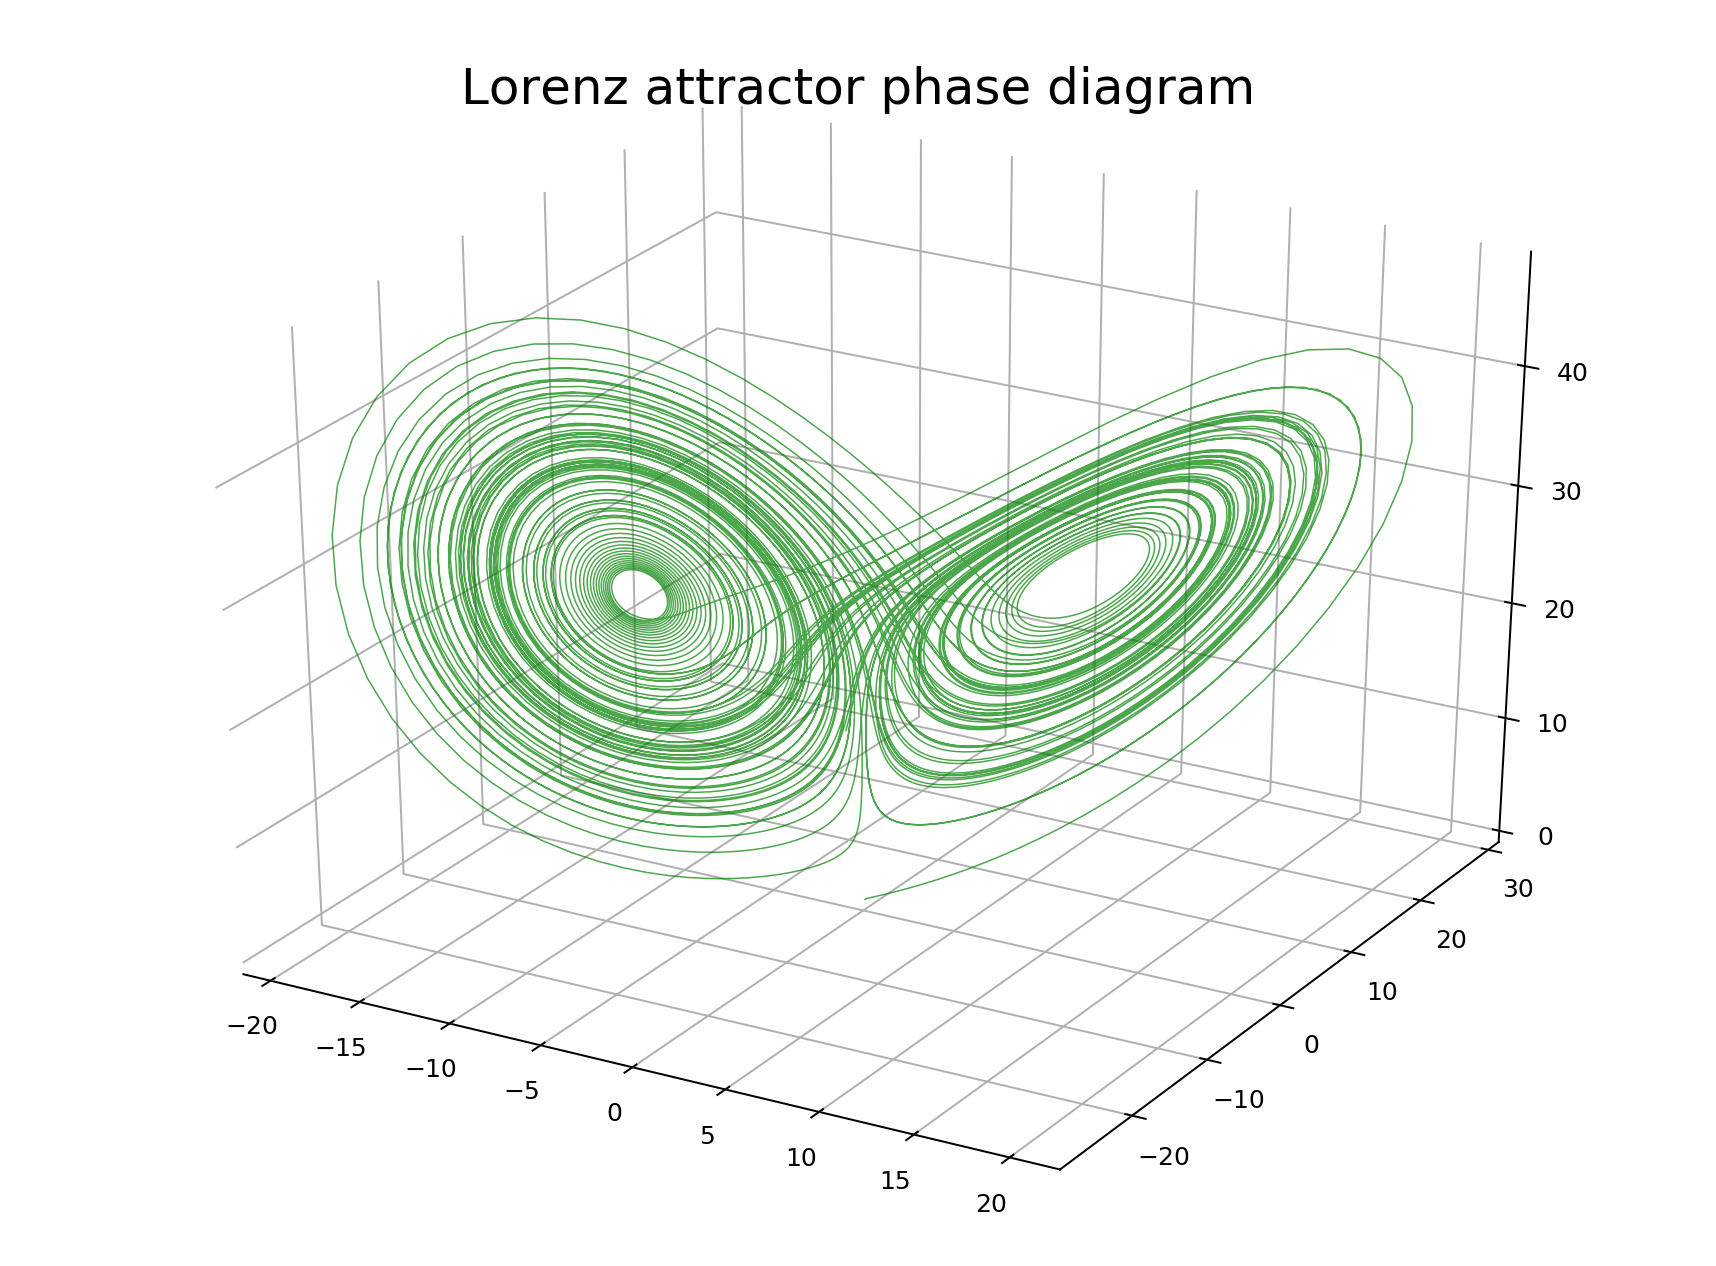
\includegraphics[width=0.5\linewidth]{ej1-pd.png}
\caption{Diagrama de fáse del atractor del sistema de Lorenz}
\end{figure}

\begin{figure}[ht!]
\centering
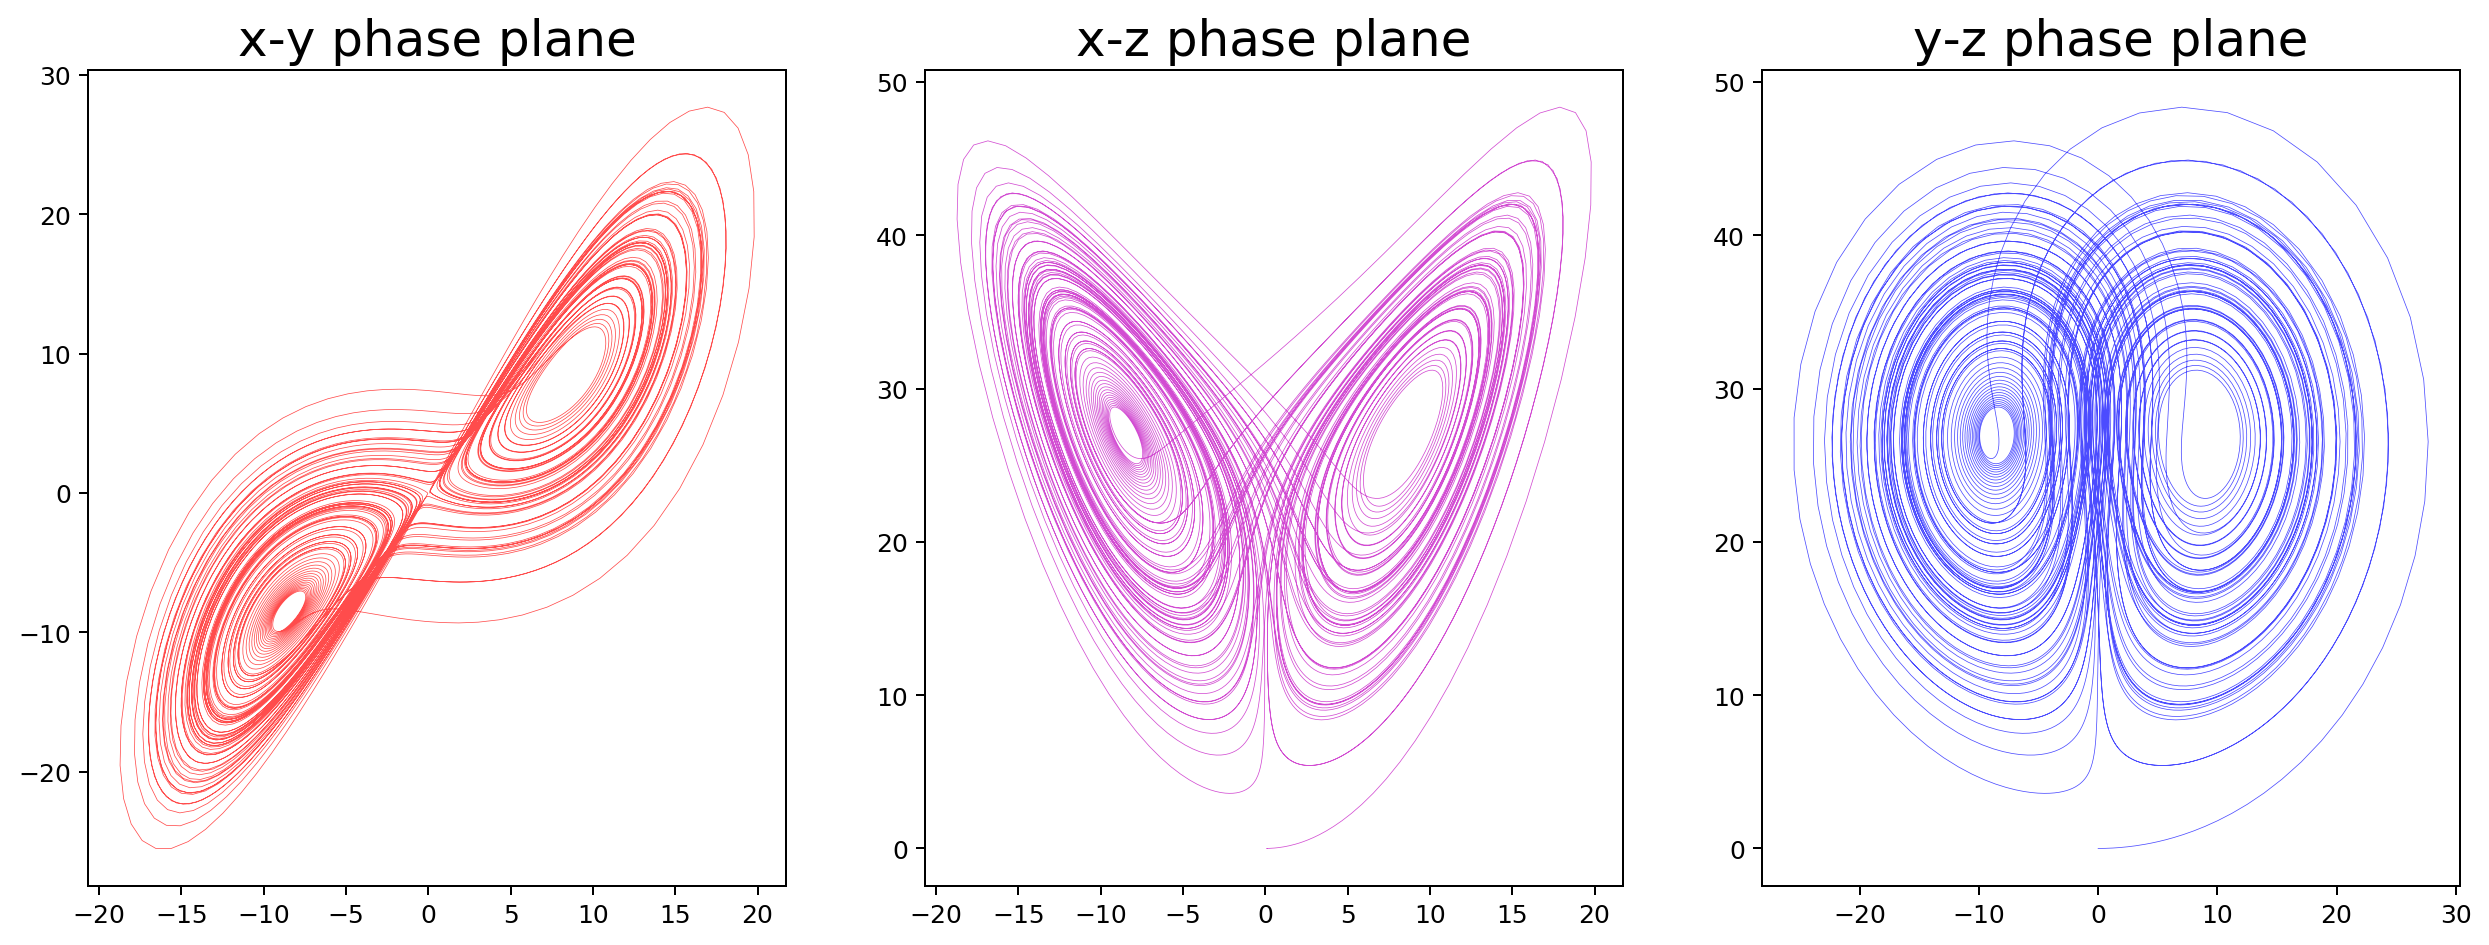
\includegraphics[width=\linewidth]{ej1-pp.png}
\caption{Retrato de fáse para los planos $xy$ $xz$ y $yz$}
\end{figure}

La animación que obtuvimos se encuentra en el repositorio de GitHub

Para el segundo punto tendremos que gráficar las variables espaciales $x$, $y$ y $z$ con respecto al tiempo $t$ en un plano bidimensional, de la misma manera que graficabamos la posición del resorte en las actividades anteriores. Esto fue realizado de la manera usual que en las practicas anteriores:

Use los arreglos que fueron extraídos de la función ODEint $x$, $y$ y $z$ y la variable de tiempo dentro del código $time\_points$ y los grafique cada posición con respecto al tiempo individualmente:
\begin{figure}[ht!]
	\begin{subfigure}[b]{0.5\linewidth}
    \raggedleft
	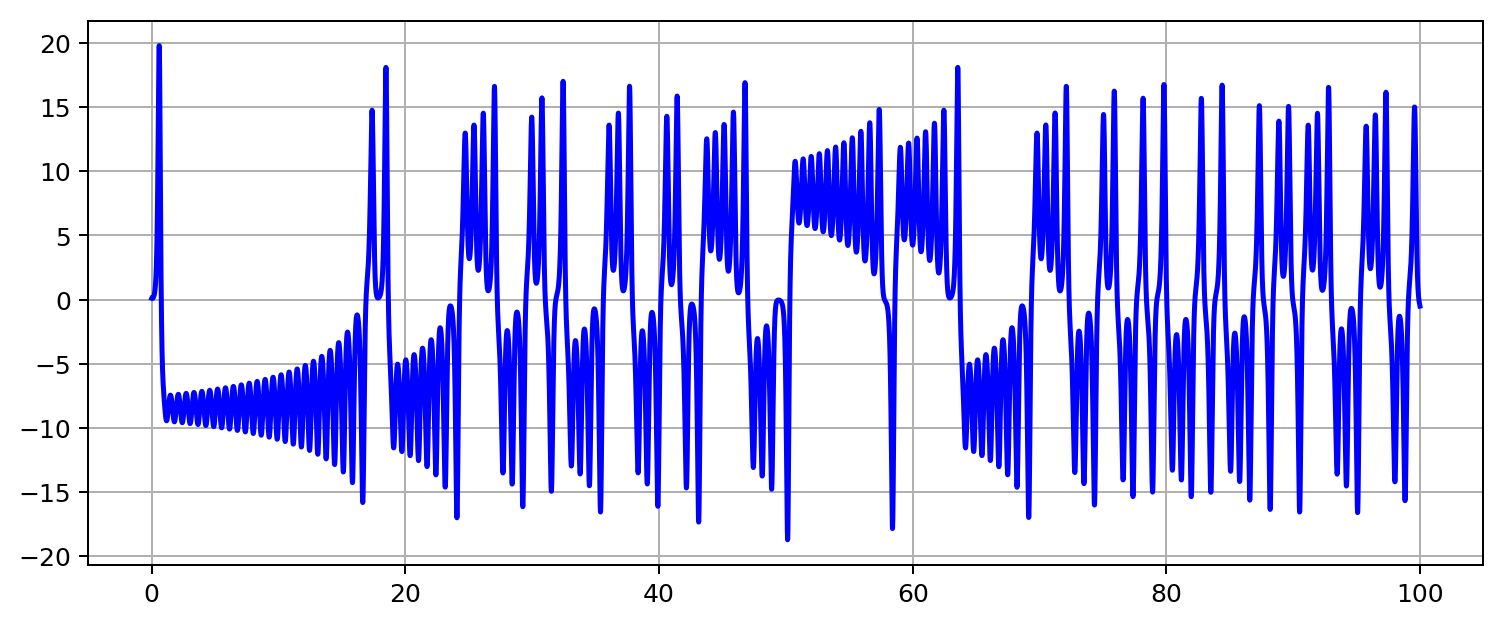
\includegraphics[width=\linewidth]{ox-t.png}
    \caption{Oscilaciones de $x$ con respecto a $t$}
	\end{subfigure}
	\begin{subfigure}[b]{0.5\linewidth}
    \raggedright
	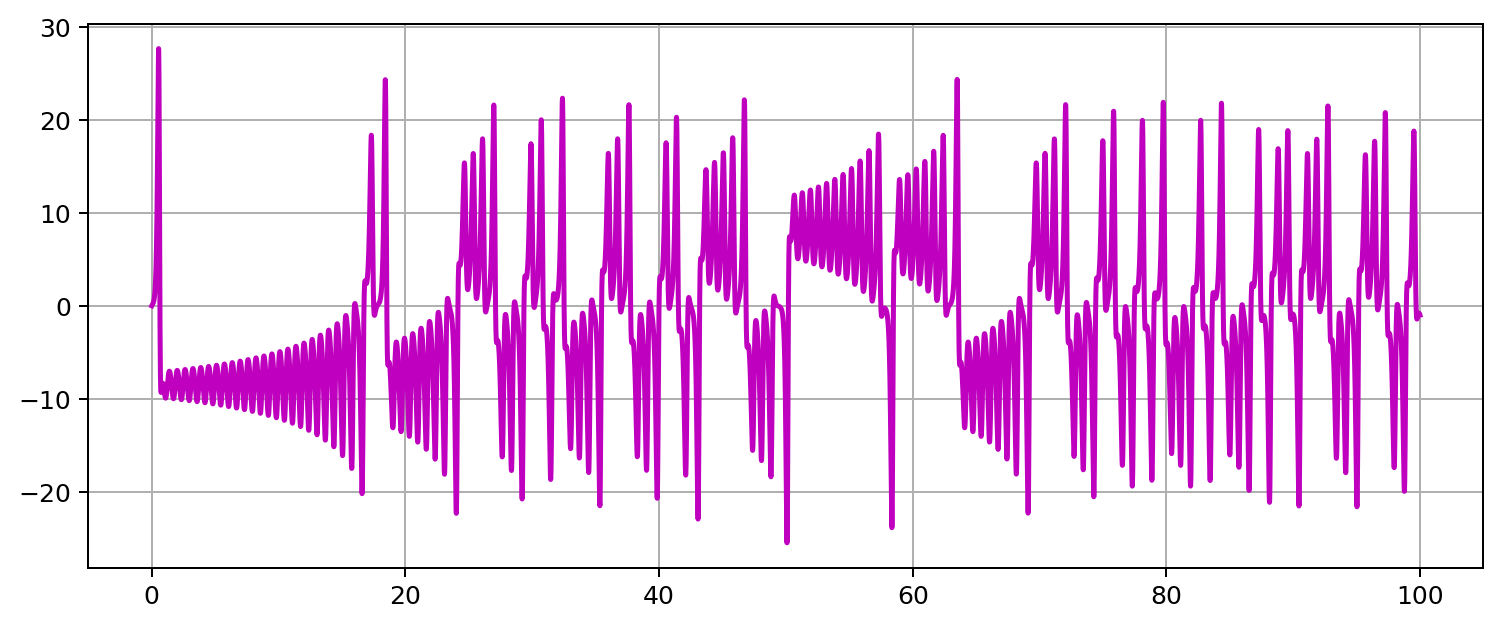
\includegraphics[width=\linewidth]{oy-t.png}
	\caption{Oscilaciones de $y$ con respecto a $t$}
    \end{subfigure}
\end{figure}
\begin{figure}[ht!]
\centering
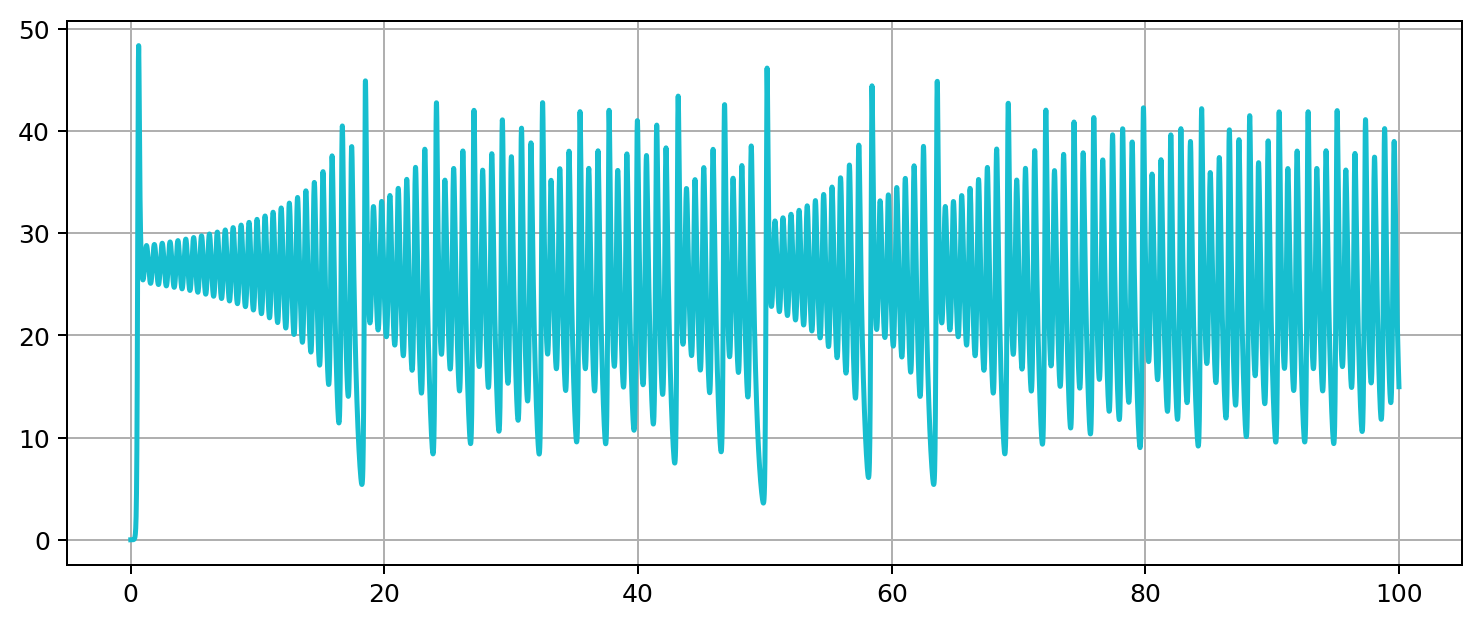
\includegraphics[width=\linewidth]{oz-t.png}
\caption{Oscilaciones de $z$ con respecto a $t$}
\end{figure}

\newpage

Y después grafique todos juntos con respecto a t simultaneamente:

\begin{figure}[ht!]
\centering
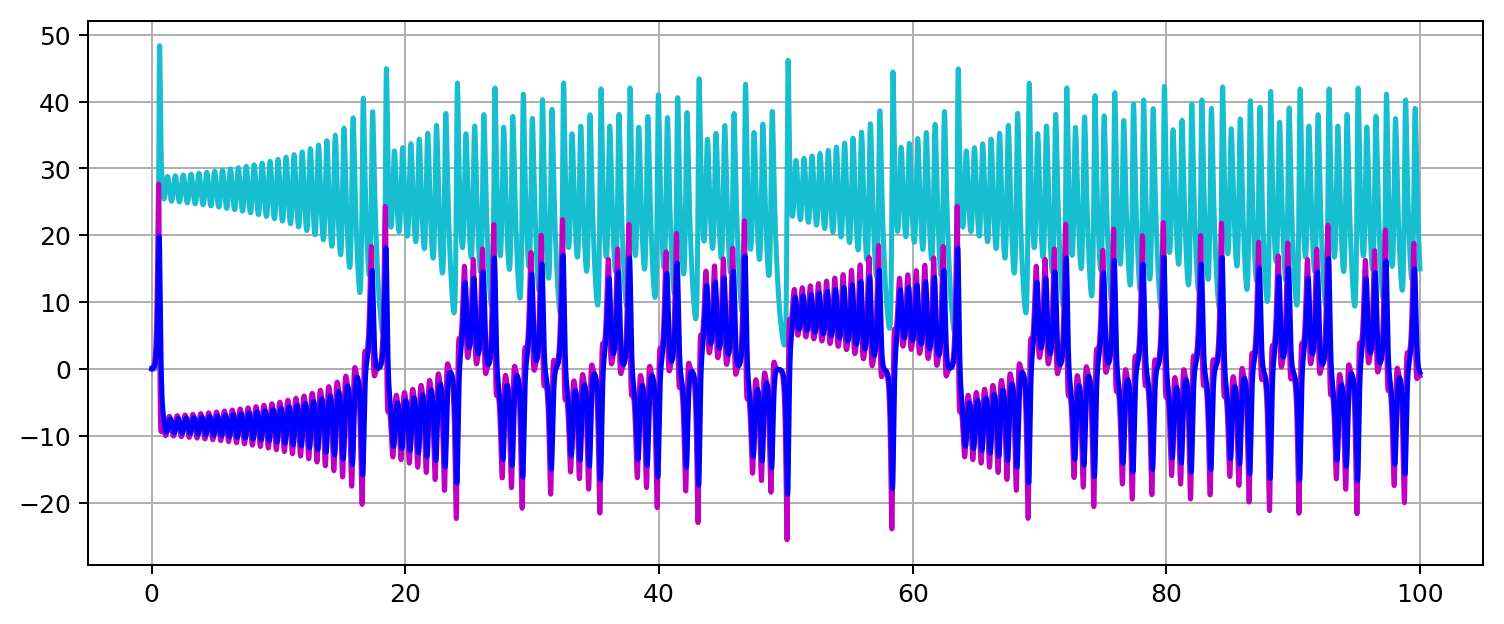
\includegraphics[width=\linewidth]{oMixed-t.png}
\caption{Oscilaciones de $x$, $y$ y $z$ con respecto a $t$}
\end{figure}

Podemos observar que la grafica de $z$ esta dada por el color \textit{cyan}, $y$ por \textit{rosa} y $x$ por \textit{azul}
~\\

Para el tercer objetivo se realizaron de nuevo las visualizaciones y animaciones del atractor, sin embargo, en este punto utilizamos los parametros $\sigma=28$, $\beta=4$ y $\rho=46.92$. Con lo que obtuve las siguientes gráficas:
\begin{figure}[ht!]
\centering
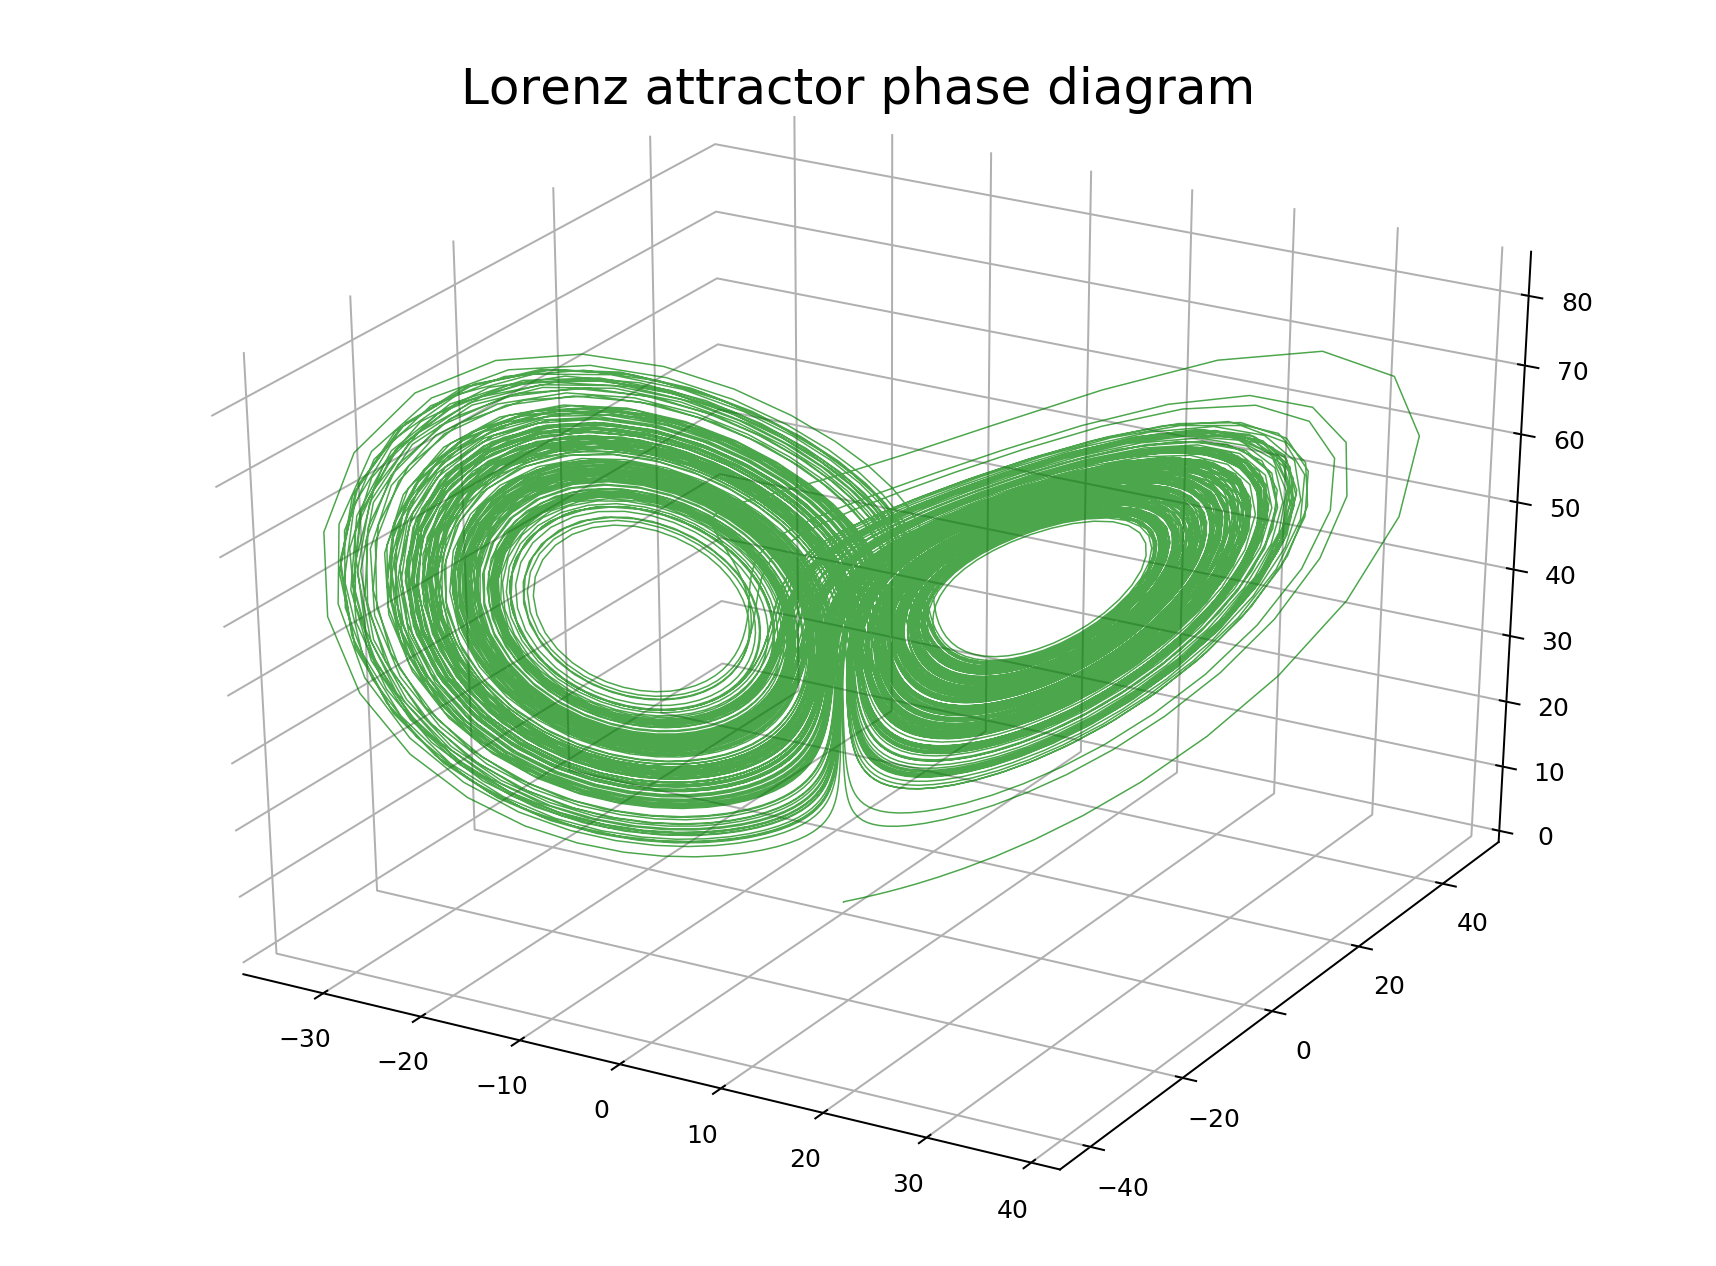
\includegraphics[width=0.5\linewidth]{ej3-pd.png}
\caption{Diagrama de fáse del atractor del sistema de Lorenz}
\end{figure}

\begin{figure}[ht!]
\centering
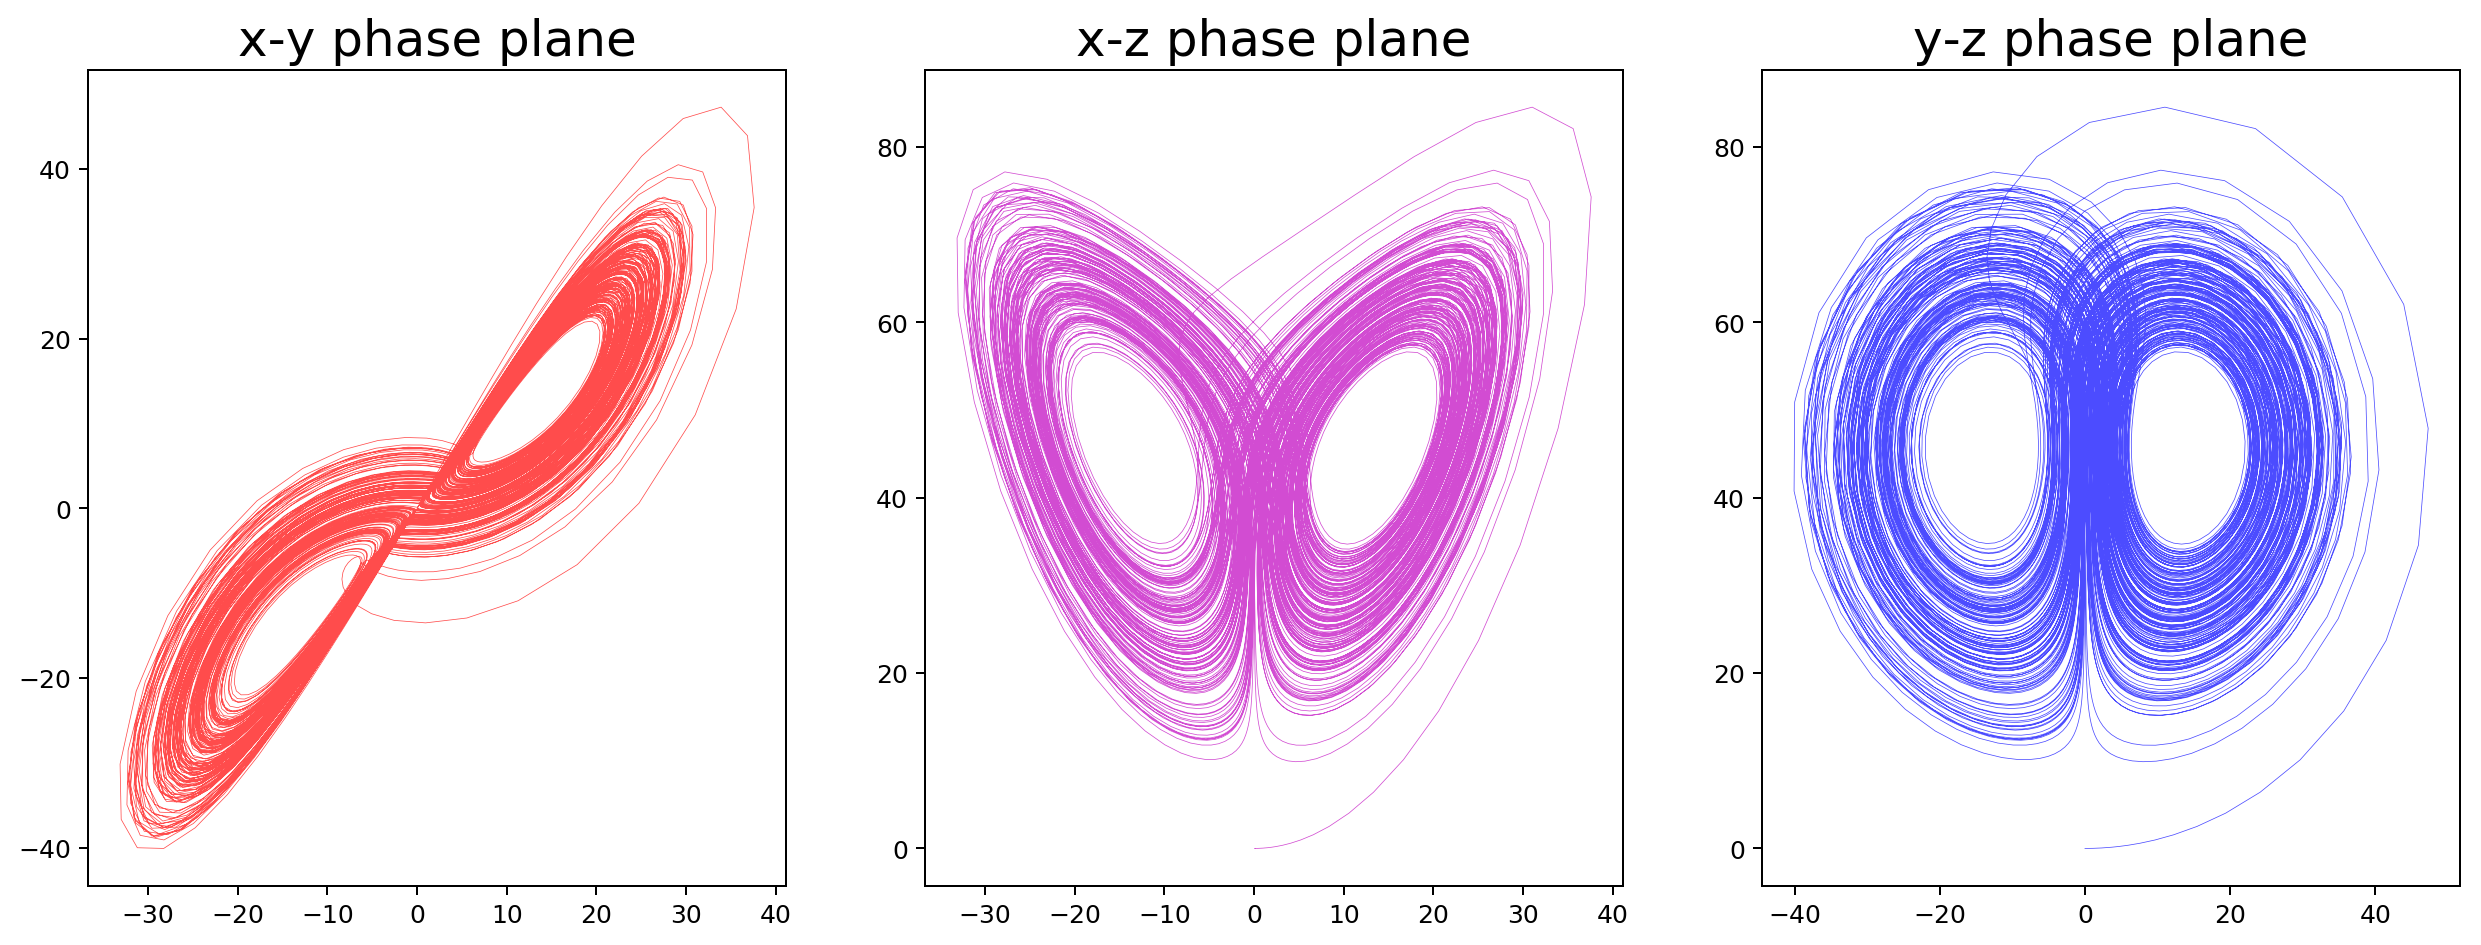
\includegraphics[width=\linewidth]{ej3-pp.png}
\caption{Retrato de fáse para los planos $xy$ $xz$ y $yz$}
\end{figure}

\newpage

La diferencia mas grande entre los atractores es el tamaño que ocupan, el de este sistema es mas "abierto"
~\\

Finalmente, para el cuarto objetivo realizamos de nuevo una visualización y animación del atractor con distintos parametros $\sigma=10$, $\beta=8/3$ y $\rho=99.96$ para observar de nuevo las diferencias. Con esto obtenemos las siguientes gráficas:
\begin{figure}[ht!]
\centering
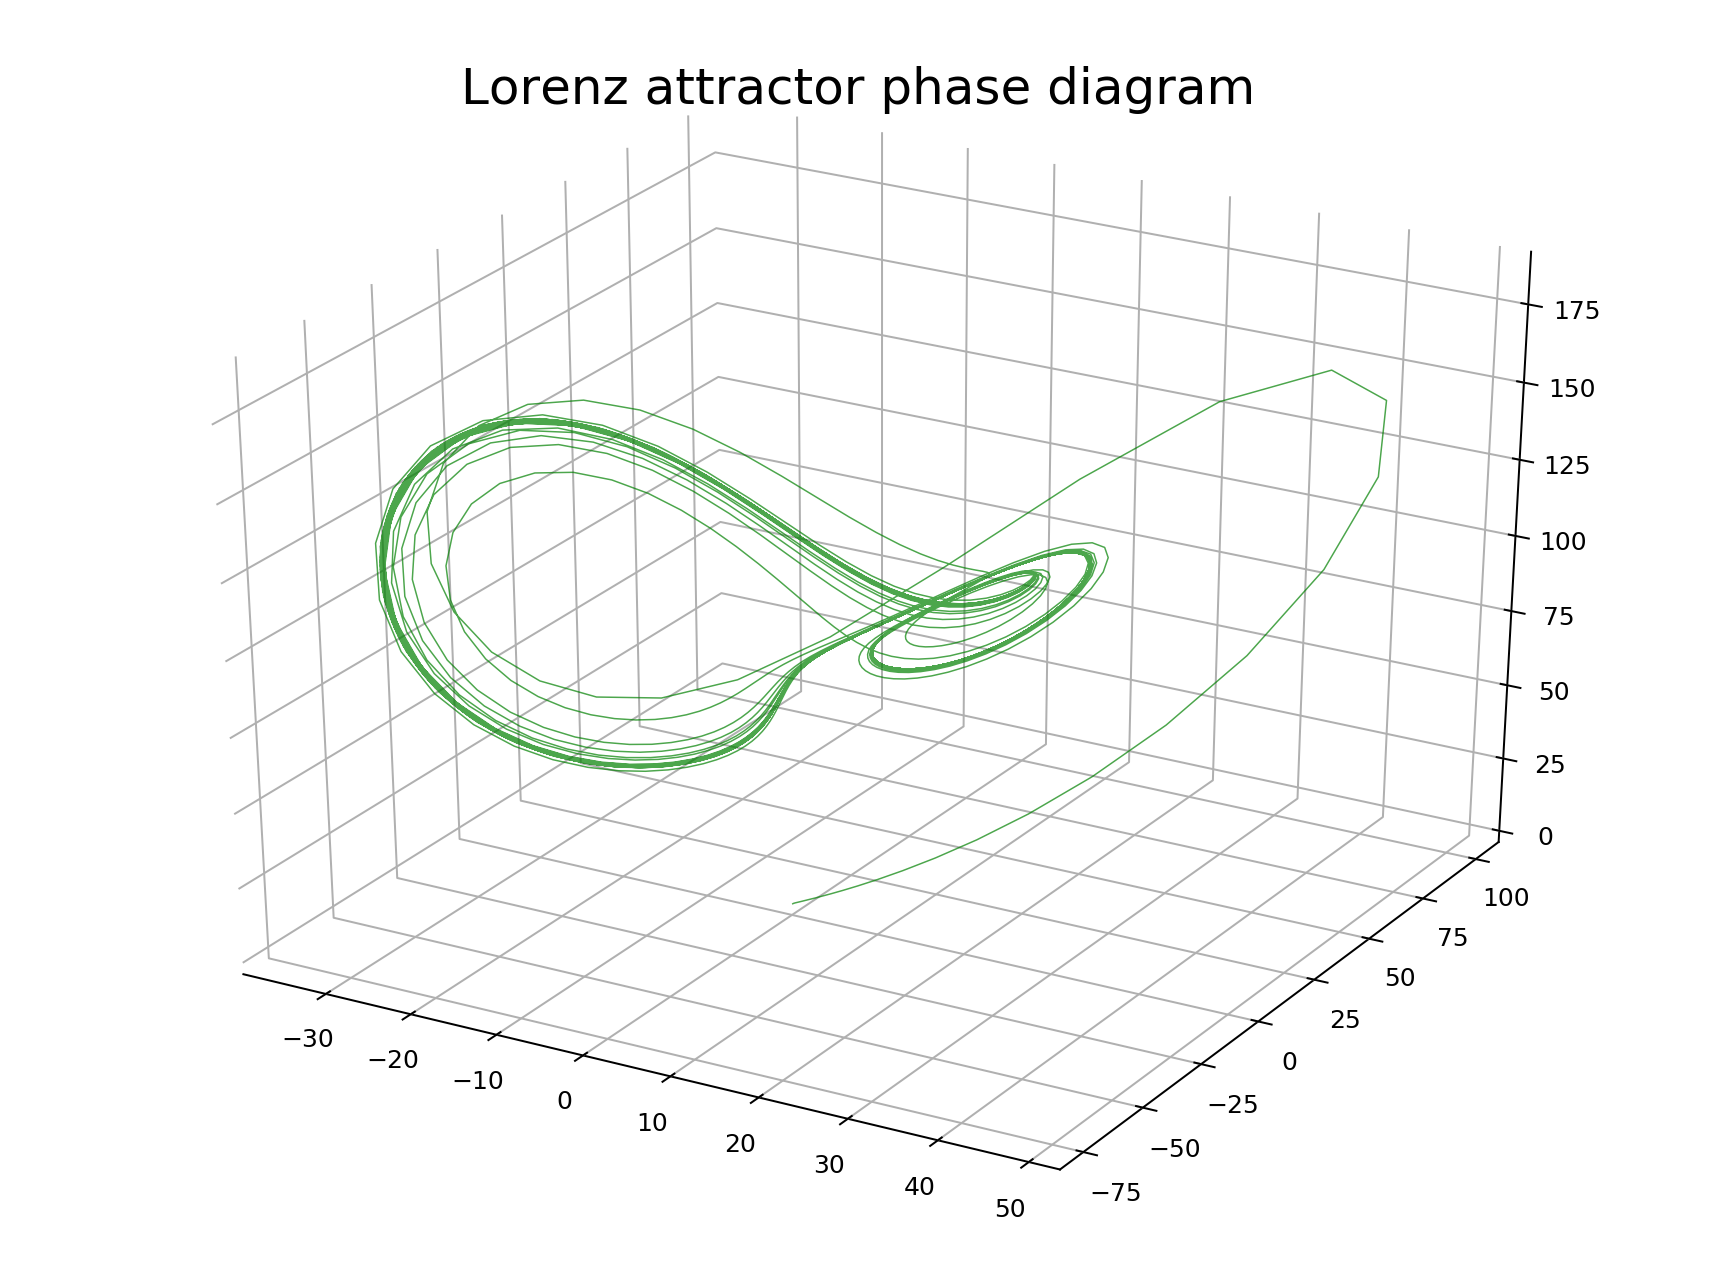
\includegraphics[width=0.5\linewidth]{ej4-pd.png}
\caption{Diagrama de fáse del atractor del sistema de Lorenz}
\end{figure}

\begin{figure}[ht!]
\centering
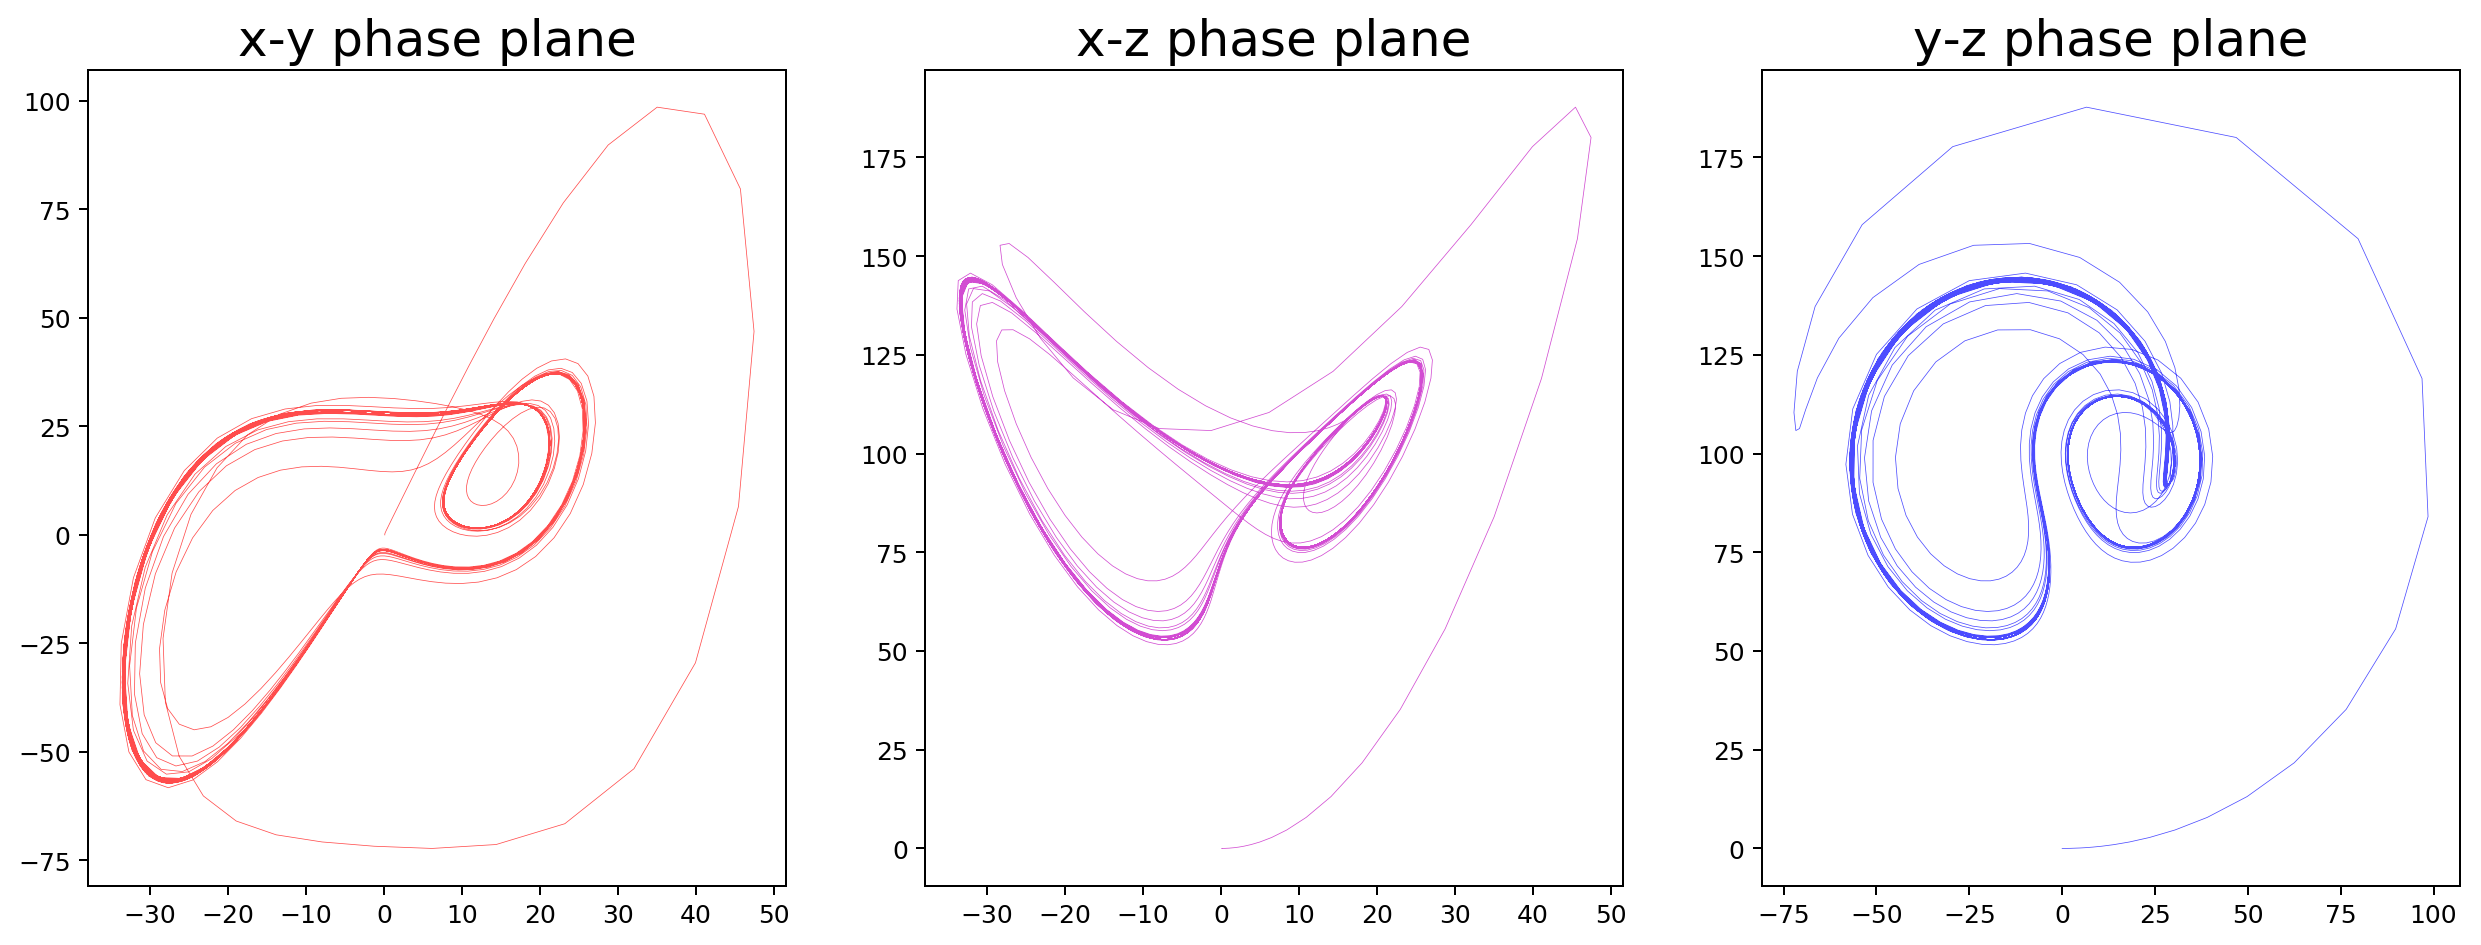
\includegraphics[width=\linewidth]{ej4-pp.png}
\caption{Retrato de fáse para los planos $xy$ $xz$ y $yz$}
\end{figure}

\newpage

Este sistema es notablemente distinto, una de las "alas" es mucho mayor a la otra, se tarda mas tiempo en llegar al atractor.

\section{Conclusión}

El atractor de Lorenz es un ejemplo de lo que conocemos como caos determinista, es un sistema de ecuaciones diferenciales bastante simplificado como para modelar adecuadamente el movimiento del viento a través de la atmósfera.

En esta evaluación observamos que es bastante facil que el atractor cambie de forma, es por esto que es caótico. Aparte de esto, aprendimos que la computadora, o python, se tardan mucho en generar, graficar y generar los datos.

\end{document}
